% arara: latexmk: { options: [ '-pdf' ] }
% arara: latexmk: { options: ['-c' ] }
\documentclass{article}
\usepackage{amsmath}
\usepackage{tikz}

\title{AP Physics C Chap 9 FRQ}
\author{Henry Beveridge}
\date{April 2, 2025}

\begin{document}

\maketitle

\section*{1.}
\subsection*{a.}
\textbf{i.} Using a spherical Gaussian surface

\begin{align*}
    \frac{q_\text{enc}}{\varepsilon_0} &= A\cdot E \\
    \frac{1}{\varepsilon_0 A} \int dq &= E \\
    \frac{1}{\varepsilon_0 4\pi r^2} \int_0^r 4\pi Cr^3 dr &= E \\
    \frac{1}{\varepsilon_0 4\pi r^2} \cdot \pi Cr^4 &= E \\
    \frac{Cr^2}{4\varepsilon_0} &= E
\end{align*}

Electric potential is then the negative integral of this field from 0 to r.
\begin{align*}
    \Delta V &= -\int E \\
    &= -\int_0^r \frac{Cr^2}{4\varepsilon_0} dr \\
    &= -\frac{Cr^3}{12\varepsilon_0}
\end{align*}

\noindent \textbf{ii. \& iii.}
\begin{center}
    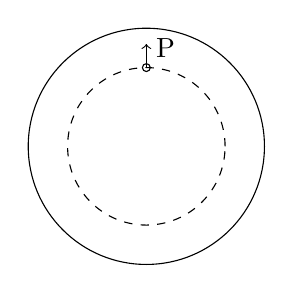
\begin{tikzpicture}
        \draw (0,0) circle (1.5);
        \draw[dashed] (0,0) circle (1);
        \draw (0,1) circle (0.05) node[anchor=south west] {P};
        \draw[->] (0,1) -- (0,1.3);
    \end{tikzpicture}
\end{center}

\subsection*{b.}
\begin{align*}
  \frac{1}{2}mv_0^2 + \frac{CR^3}{12\varepsilon_0}&= \frac{1}{2}mv^2 \\
  v_0^2 + \frac{CR^3}{6m\varepsilon_0}&= v^2 \\
  \sqrt{v_0^2 + \frac{CR^3}{6m\varepsilon_0}}&= v
\end{align*}

\section*{2.}

\subsection*{a.}
\begin{center}
    \begin{tikzpicture}
        \draw[dashed] (-4,0) -- (4,0);
        \draw[dashed] (-3,-1) -- (-3, 1) -- (-1,1) -- (-1,-1) -- cycle;
        \draw (-3,-1) circle (0.05) node[anchor=north east] {$+Q$};
        \draw (-3,1) circle (0.05) node[anchor=south east] {$+Q$};
        \draw (-1,-1) circle (0.05) node[anchor=north west] {$-2Q$};
        \draw (-1,1) circle (0.05) node[anchor=south west] {$-2Q$};

        \fill (-2, 1) circle (0.05);
        \fill (-2, 0) circle (0.05);
        \fill (-2, -1) circle (0.05);
        \fill (-1, 0) circle (0.05);
        \fill (3, 0) circle (0.05);

        \draw[->] (-2, 1) -- (-1.5, 0.75);
        \draw[->] (-2, 0) -- (-1.5, 0);
        \draw[->] (-2, -1) -- (-1.5, -0.75);

        \draw[->] (-1, 0) -- (-0.5, 0);
        \draw[->] (3,0) -- (2.5, 0);
    \end{tikzpicture}
\end{center}

\subsection*{b.}
\begin{align*}
    -\Delta V &= W_f = -\frac{kq}{r} \\
    &= - \left(2\cdot \frac{kQ}{s\sqrt2} - 2\cdot \frac{k2Q}{s\sqrt2}\right) \\
    &= 2\frac{kQ}{s\sqrt2}
\end{align*}

\subsection*{c.}
\begin{center}
    \begin{tikzpicture}
        \draw (0,-4) -- (0,4);
        \draw (0,0) -- (6,0);
        \node[anchor=east] at (0,0) {$0$}; 
        \node[anchor=east] at (0,4) {$U$};

        \draw (2,0.1) -- (2,-0.1) node[anchor=north] {$\frac{s}{2}$};

        \draw[domain=0:2] plot (\x,{0.5*ln(-\x+2.2)-1});
        \draw[domain=2:6] plot (\x,{0.5*ln(\x-1.5)-1.5});
    \end{tikzpicture}
\end{center}

\subsection*{d.} Yes, it is consistent because electric potential is negative at $x=0$, and at $x=5.5s$ it is also negative but closer to zero. 

\section*{3.}
\subsection*{a.} Put the negative end of the voltmeter in the center of the disk. Then, for multiple trials, put the positive end in the paper at varying distances away from the center, and record the measurment on the voltmeter. Plot distance on x-axis and voltage on y-axis.

\subsection*{b.} Plot $\frac{1}{r^2}$ on x-axis and voltage on y-axis.

\section*{4.}
\subsection*{a.}
$V_1=V_2$ Because all of the charge is still the same distance away from the point, the direction doesn't matter.

\subsection*{b.}
\begin{align*}
    V_2 &= \int \frac{kdq}{r} \\
    &= \frac{k}{r} \int_0^L \lambda_2dx \\
    &= \frac{k}{r} \int_0^L \lambda_0\frac{x}{L}dx \\
    &= \frac{k\lambda_0L}{2R}
\end{align*}

\subsection*{c.}
\begin{align*}
    Q &= \int_0^L \lambda_0 \frac{x}{L} dx \\
    &= \frac{\lambda_0 L}{2}
\end{align*}

Yes, it's accurate because then the equation is just $\frac{kQ}{r}$, or the equation for electric potential. 

\end{document}
